\documentclass[12pt]{article}
\usepackage[utf8]{inputenc}
\usepackage{graphicx}
\renewcommand{\figurename}{Ábra.}

\begin{document}

\section{Alapok}

\subsection{Neurális hálók}

A neurális hálók biológiai indíttatású programok, amelyek a biológiai neurális hálózat néhány hasznos tulajdonságát modellezik.

\subsubsection{Alapvető felépítése}

A neurális hálók mindössze bonyolult, sok paraméteres, többdimenziós függvények, amelyek egy $n$ dimenziós inputhoz $k$ dimenziós outputot határoznak meg.

Például egy emberhez, pontosabban annak adataihoz hozzárendelnek egy betegséget olyan módon, hogy a négy output közül az veszi fel az $1$ értéket amely betegség a függvény “válasza”, az összes többi (betegséghez tartozó) output pedig $0$. A hálózat tehát meg tudja becsülni, hogy az illető milyen betegségben szenved.

\begin{figure}[h!]
  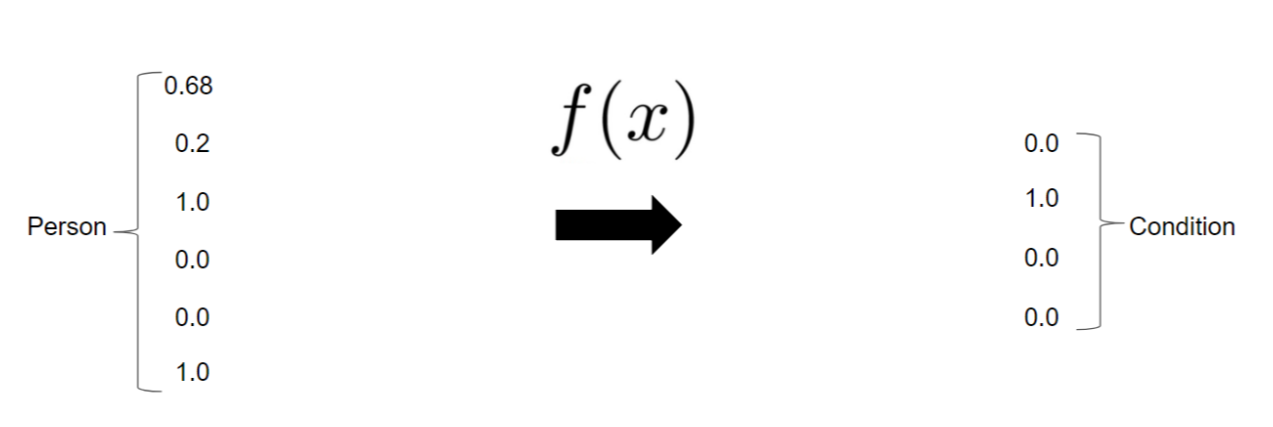
\includegraphics[width=\linewidth]{fgv.png}
  \caption{Általános nézet}
\end{figure}

Ez így elég egyszerűen hangzik, mivel még nem tárgyaltunk arról, hogy ez a függvény hogyan működik, és honnan tud néhány adatból betegségre vonatkozó következtetéseket levonni. A kérdés tehát, hogy hogyan határozzuk meg ezt a függvényt. Legyen a függvény egy neurális háló:

\begin{figure}[h!]
  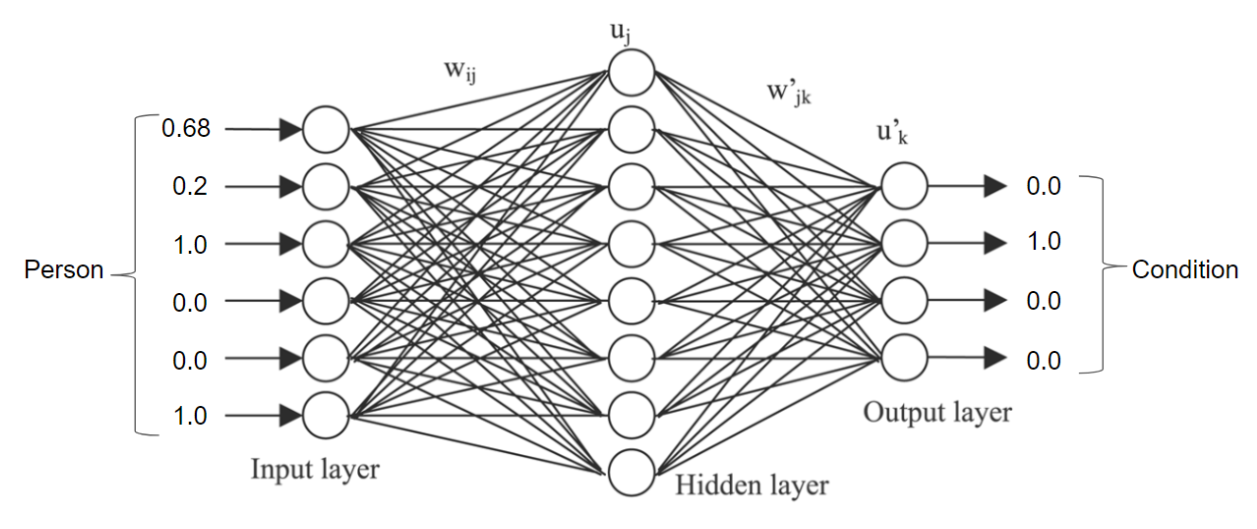
\includegraphics[width=\linewidth]{fgv_network.png}
  \caption{Konkrét neurális háló}
\end{figure}


A neurális háló tulajdonképpen egy súlyozott gráf, melynek n darab csúcsa a bemeneteket reprezentálja, k darab csúcsa pedig a kimeneteket. Az n és k csúcsok halmazát rendre input és output layernek (rétegnek) nevezzük, azonban a maradék csúcsok több kisebb halmazra bonthatóak, az úgynevezett hidden (rejtett) rétegekre. 

Egy egyszerű neurális háló tehát L darab layerből áll, melyek közül az input és output layerek speciális funkciót látnak el. A rétegeknek van egy rögzített sorrendje, amely egy neurális hálónak fix tulajdonsága, sosem változik meg. Sorrendben az első réteg az input layer, amit néhány rejtett réteg követ, majd egy output layer zárja a listát.

Minden réteget neuronok egy halmaza alkot. Ezek a gráf csúcsai. Az élek kizárólag a szomszédos layerek neuronjai között futhatnak. A gráf összes éléhez tartozik továbbá egy-egy valós számértékű súly.

A neuronoknak van egy úgynevezett aktivációs értékük, amely minden pillanatban az az érték, amelyet utoljára - manuálisan vagy automatikusan - beállítottunk neki. Egy neuron aktivációs értéket úgy határozzuk meg, hogy vesszük a neuron rétegét megelőző layer azon neuronjait, amelyekkel össze van kötve, majd vesszük ezeknek a lineáris kombinációját a hozzájuk tartozó élek súlyaival. Ehhez még hozzáadunk egy bias értéket, amely magához a vizsgált neuronhoz tartozik és szintén egy 0 és 1 közé eső skalár.
Ezután még az így kapott összegre alkalmazunk egy úgynevezett aktivációs függvényt, amely ugyancsak a neuronhoz tartozik (bár általában egy rétegben minden ez neuronra azonos).

\begin{figure}[h!]
  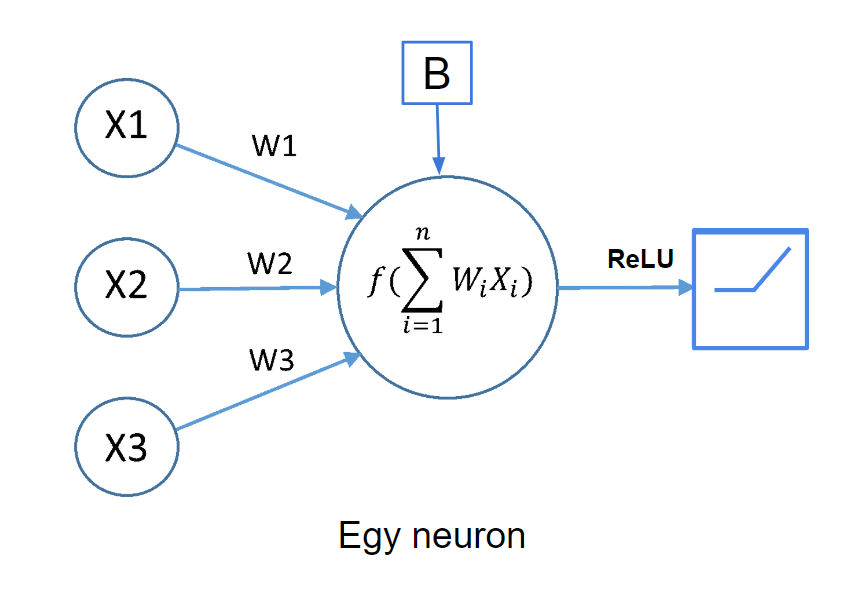
\includegraphics[width=\linewidth]{neuron.png}
  \caption{Egy neuron}
\end{figure}

Az aktivációs függvény rendeltetése, hogy a lineáris kombináció és a bias hozzáadása után keletkezett - várhatóan 1-nél nagyobb - számot visszaskálázzuk a [0-1] intervallumba.
Többféle aktivációs függvény is használhatunk, leggyakoribbak a:

\begin{itemize}  
	\item Sigmoid: $f(x) = \frac{e^x}{e^x+1}$ 
	\item ReLU : $f(x) = max(0,x)$
\end{itemize}

Az input neuronoknál nem tudjuk kiszámolni a lineáris kombinációt, mivel nincs előző réteg, az ő esetükben egyenesen az aktivációs értéket állítjuk be inputnak. Miután minden input neuron aktivációs értékét beállítottuk látható, hogy az egész hálón végig fog menni egy változás, mert iteratívan minden réteget megelőző réteg megváltozik, tehát a maga a réteg is megváltozik.

Arra, hogy a neurális háló súlyai és biasei milyen értékek kezdetben, több lehetőség is van:
\begin{itemize}  
	\item mindegyik 0 vagy mindegyik súly 1
	\item valamilyen eloszlásból generált random számok
	\item fájlból betöltött értékek (tanítás folytatása esetén)
\end{itemize}

Ha tehát megadunk egy inputot, akkor az meghatározza az output layer neuronjainak konkrét aktivációs értékeit. Ez az érték lista a függvény kimenete. Érezhető, hogy ha egyszerűen tetszőleges inputokra rá eresztjük ezt a kalkulációt, akkor az nagyjából random outputokat fog generálni. A tanítás alapú mesterséges intelligencia algoritmusoknál azonban rendelkezésünkre állnak helyes input-output párok egy listája, vagyis egy inputhoz már kétféle outputot is tudunk mondani: az adathalmaz outputját, illetve ezt a randomnak tűnő outputot amit a háló generál.

\begin{figure}[h!]
  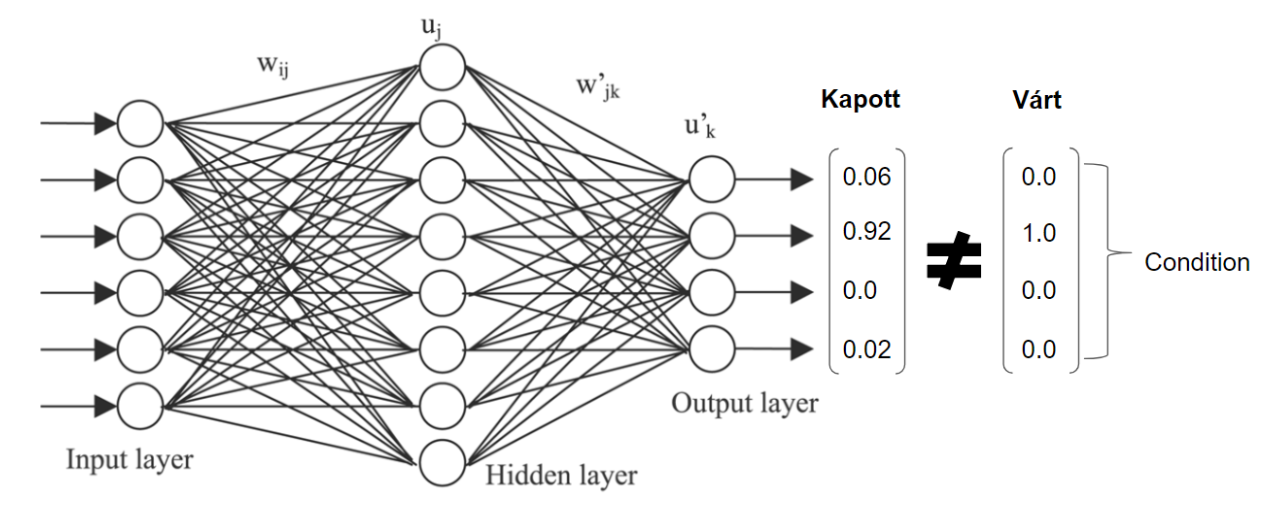
\includegraphics[width=\linewidth]{kapott_vart.png}
  \caption{A kapott érték nem egyezik meg a várttal}
\end{figure}

Ha a hálónk, nem képes a várt kimenetet megközelíteni, akkor a mi megközelítésünkben hibázik. Olyan módon kell változtatni a neurális háló súlyait és biaseit, hogy ezek a hibák minimálisak legyenek, hiszen ekkor a predikció is pontos. Ennek megvalósításához elengedhetetlen, hogy a hibát számszerűsíteni tudjuk.

Azon függvényeket, melyek egy $t$ várt és egy $x$ kapott vektorhoz kiszámítanak egy hibát, $\lambda(x,t)$ loss fuctionöknek nevezzük.

\subsection{Backpropagation}

Minden input-output párra meg kell változtatni a súlyokat és biaseket, mindegyiket más mértékben. Minél jobban felelős egy súly a hibáért annál jobban meg kell azt változtatni. A felelősség eldöntéséhez backpropagáljuk a hibát, vagyis a hiba vektort aktivációs értékként beállítjuk az output layernek és fordított irányban végrehajtjuk a rétegek neuronjainak aktivációját.
Például: ha a hibavektor egyik neuronja 0, tehát az adott értéket pontosan jósolta meg a háló, akkor a hozzá tartozó súlyoknak semmilyen felelőssége nincsen a hibában, ezért a 0 érték propagálódik vissza rajtuk.

\begin{figure}[h!]
  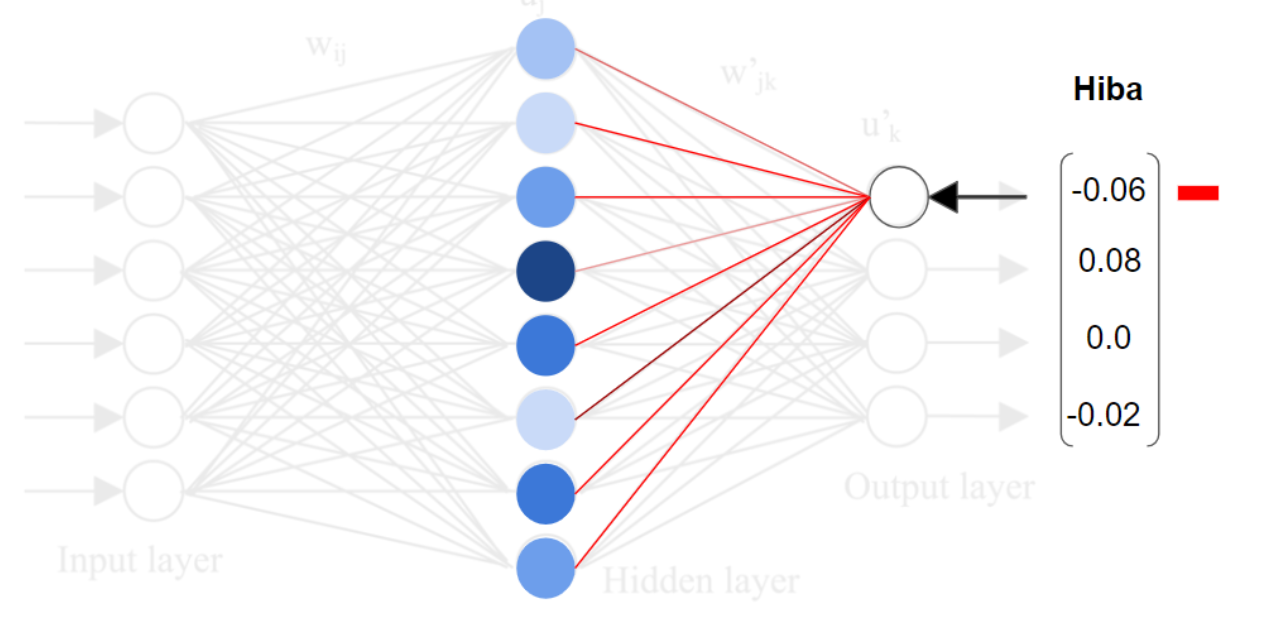
\includegraphics[width=\linewidth]{backprop_single_error.png}
  \caption{Egy neuron felelőssége a mögötte lévő rétegben}
\end{figure}

A felelősséget végül nem a súlyokon, hanem a neuronokon fogjuk realizálni. A backpropagation végeztével tehát minden neuronon lesz egy felelősség érték.

\begin{figure}[h!]
  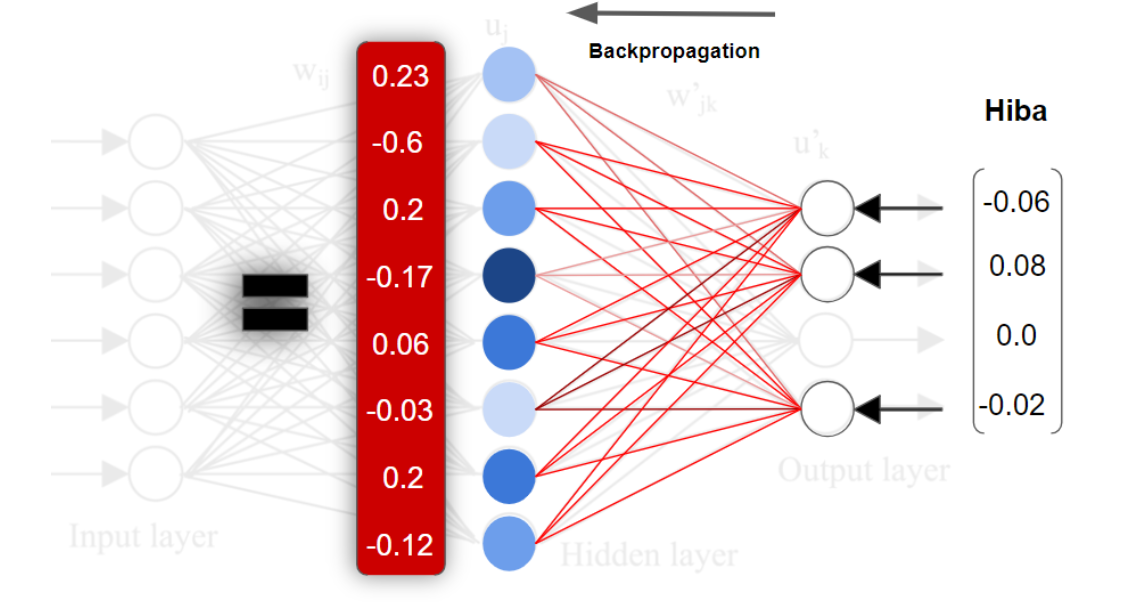
\includegraphics[width=\linewidth]{backprop_all_error.png}
  \caption{Egy réteg teljes felelőssége a mögötte lévő rétegben}
\end{figure}

A neuronokon azonban nincs mit megváltoztatni, csak a súlyok és biasek változtatása lehetséges. A súlyok megváltoztatására a képlet az alábbi:
$$ w_{new} =  w_{old} + b_{error} * a_{activation} * l $$
ahol $w$-vel jelölt értékekkel, a megváltoztatás előtti, illetve utáni súlyokat jelöljük, $a$ az - irányított - él kezdőpontja, $b$ pedig a végpontja, $l$ pedig a tanulás sebessége.

A backpropagationt több input-output párra is el kell végezzük, ekkor visszünk be információt a rendszerbe arról, hogy mely párokat tartunk helyesnek, és végül az algoritmus ebből fogja ezt a véges tudását általánosítani bármilyen - korábban nem látott - inputra. Azt a folyamatot amikor az összes kívánt párra lefuttatjuk a backpropagationt $epochnak$ nevezzük. 

Ha általában meg szeretnénk mérni azt, hogy a jelenlegi háló milyen hatásfokkal tud perdiktálni, akkor nem elég a tanítás közben megnézni, mekkora hibákat backpropagál program, mivel az egész háló arra van optimalizálva, hogy erre a konkrét tanító adathalmazra hatékonyan működjön. Éppen ezért a tanítás előtt két részre osztjuk az adathalmazt:

\begin{itemize}  
	\item tanító adatok (train set): amelyeken végrehajtuk a backpropagationt, 1 epochban minden adatra egyszer
	\item validációs adatok (validation set): minden epoch végén leteszteljük ezekre az adatokra, hogy mekkora hiba keletkezik, backpropagationt viszont nem futtatunk a hibákon
\end{itemize}

A backpropagationt a gyakorlatban nem szokás minden egyes tanító adatpár után lefuttatni, hanem egyszerre több adatnak az aggregált hibáját vezetjük vissza a súlyok megváltoztatásához. Ez párhuzamosításra ad lehetőséget, amely nagy mértékben tudja csökkenteni a futásidőt.

Az epoch szám megválasztásánál figyelni kell arra, hogy a hálót ne tanítsuk túl (overfitting). vagyis ne specialázájuk rá túl nagy mértékben a tanító adathalmazra, valamint ennek ellenkezője, az alul tanítás (underfitting) is pontatlanságot eredményez, amikor egyszerűen a háló még a tanító adatokra sem képes megfelelő pontossággal prediktálni.

\subsection{Konvolúciós hálók}

A konvolúciós hálókat a legtöbb esetben kép klasszifikációra használják, vagyis háló feladata az, hogy az inputjára kapott képről (egy előre meghatározott listából) elndöntse, hogy  mi szerepel rajta (például: kutya vagy macska). Ha $n$ féle osztályt klasszifikál a háló, akkor $n$ darab output neuronja van, a kép inputra adott válasza pedig egy $n$ elemű eloszlás arról, hogy a háló jelenlegi tudása szerint melyik osztály előfordulását milyen valószínűnek tartja.

A korábbiakban általánosságban tárgyaltuk a neruális hálókat, csak annyit állítottunk, hogy a szomszédos rétegek neuronjai vannak egymással kapcsolatan. Általános esetben egy réteg minden neuronja összeköttetésben áll az őt megelőző réteg mindenen neuronjával. Az ilyen réteget teljes-összeköttetésű rétegnek nevezik, a kizárólag ilyeneket tartalmazó hálók pedig sűrű (dense) hálók.

Kép inputok esetén a sűrű hálók, azonban nem használják ki a képben rejlő azon információt, hogy bizonyos pixelek közelebb vannak egymáshoz mint más pixelek, hiszen az input neuronok szerepe a teljes-összeköttetés miatt felcserélhető. Egy sűrű hálónak ebben az esetben tehát még azt is meg kell tanulnia, hogy mit jelent képnek lenni (összefüggő egyszínű tartományok az egymáshoz közeli pixeleknél, néha éles színváltás).

Ezt a problémát oldják meg a konvolóciós hálók úgy, hogy nem kizálagosan teljes-összeköttetésű rétegeket alkalmaznak, hanem egyéb speciális rétegeket is:

\begin{itemize}
  \item Konvolúciós réteg
  \item Pooling réteg
\end{itemize}

A konvolúciós hálók általában úgy vannak felépítve, hogy néhány konvolúciós rétegenként tartalmaznak egy pooling réteget, majd a kimeneti réteg - amikor már csak egy 1 dimenziós vektort várunk - egy teljes-összeköttetésű réteg.

A súlyok javítására ugyanúgy a backpropagation algoritmus használjuk.

\subsubsection{Konvolúciós réteg}

A konvolúciós hálók rétegeit elsősorban három dimenziósnak képzeljük el. Színes kép esetén például az input réteg három dimenziója: a kép magassága, szélessége és a pixelek színe. A réteg példában szereplő szín dimenzióját a réteg mélységének nevezzük.

A konvolúciós rétegek $K$ darab szűrőből (filterből) állnak, melyek $n\times n$-es súly mátrixok, ahol $n$ általában egy kis egész szám, például 3, paraméter. Maga a réteg pontosan $K$ mélységű, minden filter egy alréteget határoz meg.

A réteg neuronjainak aktivációját a következőképpen számoljuk ki: az előző rétegnek vesszük az összes $n\times n\times d$-s ablakát, ahol $d$ az előző réteg mélységét, az ablak pedig egy neuronokból képezhető téglatestet jelöl, első réteg esetén például a középső $3\times3$ pixelt és színeiket. Minden ilyen ablak $K$ darab neuron aktivációját határozza meg, tehát minden filterhez egyet. A $k$. filter esetén az aktiváció az ablak neuron aktivációinak a filter súlyaival vett lineáris kombinációja lesz. Ezt hívják konvolúciónak.

\begin{figure}[h!]
\begin{center}
  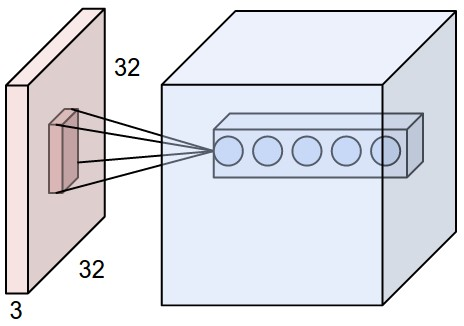
\includegraphics[width=0.5\linewidth]{depthcol.jpg}
  \caption{Egy konvolúciós réteg összes neuronja egy ablak pozícióhoz}
\end{center}
\end{figure}

Egy konvolúciós rétegnek vannak egyéb - kevésbé fontos - paraméterei is a filterek száma és az ablakméret mellett, például az hogy az ablak eltolásánál hány neuronnyit lépünk (stride) vagy az ablak viselkedése a neuronmátrix határán (padding).

\subsubsection{Pooling réteg}

Pooling rétegeket általában két konvolúciós réteg között szoktak használni a későbbi rétegek méretének csökkentése céljából. Ez csökkenti a súlyok számát, így gyorsítja a futást, azoban ez a múvelet infromáció veszteséggel jár. Ha a képes analógiát tekintjuk, ez egy veszteséges képméret csökkentésnek felel meg (lásd \ref{pool} ábra). A konvolóciós rétegeknél is (megfelelő padding típussal) csökken a méret, a pooling réteg esetében általában nagyságrendileg felezni szokás a szélességet és magasságot.

\begin{figure}[h!]
\begin{center}
  \label{pool}
  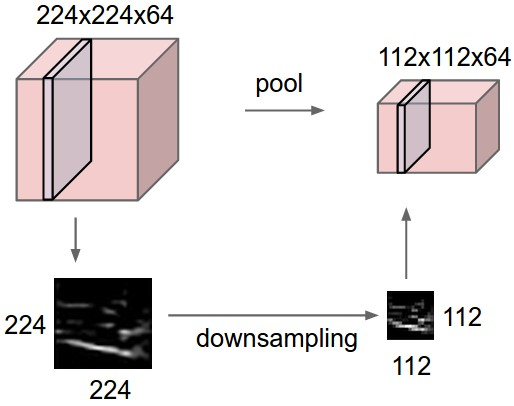
\includegraphics[width=0.5\linewidth]{pool.jpeg}
  \caption{Egy konvolúciós réteg összes neuronja egy ablak pozícióhoz}
\end{center}
\end{figure}

\subsection{Autoencoderek}

Az autoencoderek olyan speciális neurális hálók, amelyek képesek az input rétegükre érkező adatot egy rövid kóddá tömöríteni (encode), majd abból a kódból az eredeti inputot visszaállítani (decode). Ezt a két funkciót egyetlen hálóval valósítjuk meg, azonban a hálón belül jól elkülönül a két rész: a rétegek első fele végzi el a kódolást, a második fele pedig a dekódolást. Az encodernek folyamatosan csökkennek, a decodernek pedig növekszenek a rétegeik mérete, ahogy ezt a \ref{AE_arch2} ábra mutatja. Az encode-olás és decode-olás egymás utáni elvégzése elméletben egy identitás. A tanítás során ezért a kimeneten várt érték maga az input, nincs szükségünk adatpárokra, pusztán kódolandó adatokra. A háló tanításásához szükséges hibát tehát a rekonstrukcó hatásfoka fogja meghatározni.

A háló "közepén" elhelyezkedő legkisebb méretű réteget reprezentációs vagy látens rétegnek nevezzük, a kiértékelés során az itt megjelenő aktivációs értékek vektora jelenti a kódot. Ez a kód valóban az inputra érkező adatot reprezentálja, hiszen az adatból (az encoderrel) elő tudjuk állítani a kódot, a kódból pedig (a decoderrel) vissza tudjuk állítani az adatot.

A \ref{AE_arch2} ábrán látható input egy kép, az MNIST adathalmazból, mely nagy mennyiségű alacsony felbontású képeket tartalmaz rajzolt számjegyekről. Látható, hogy a (már előzőleg betanított) háló kis hibával, de képes rekonstruálni a képet (hiszen a kimenet valóban hasonlít a bemenetre). A kép vektor reprezentációja (kód) a középső két neuronjának aktivációjából olvasható ki. A háló (pontosabban a decoder) tehát képes volt 2 számból előállítani $784$ számot (egy $28\times 28$ pixel méretű képet), vagyis az autoencoderek nem csak kódolásra, hanem tömörítésre is alkalmasak.

\begin{figure}[h!]
\begin{center}
  \label{AE_arch2}
  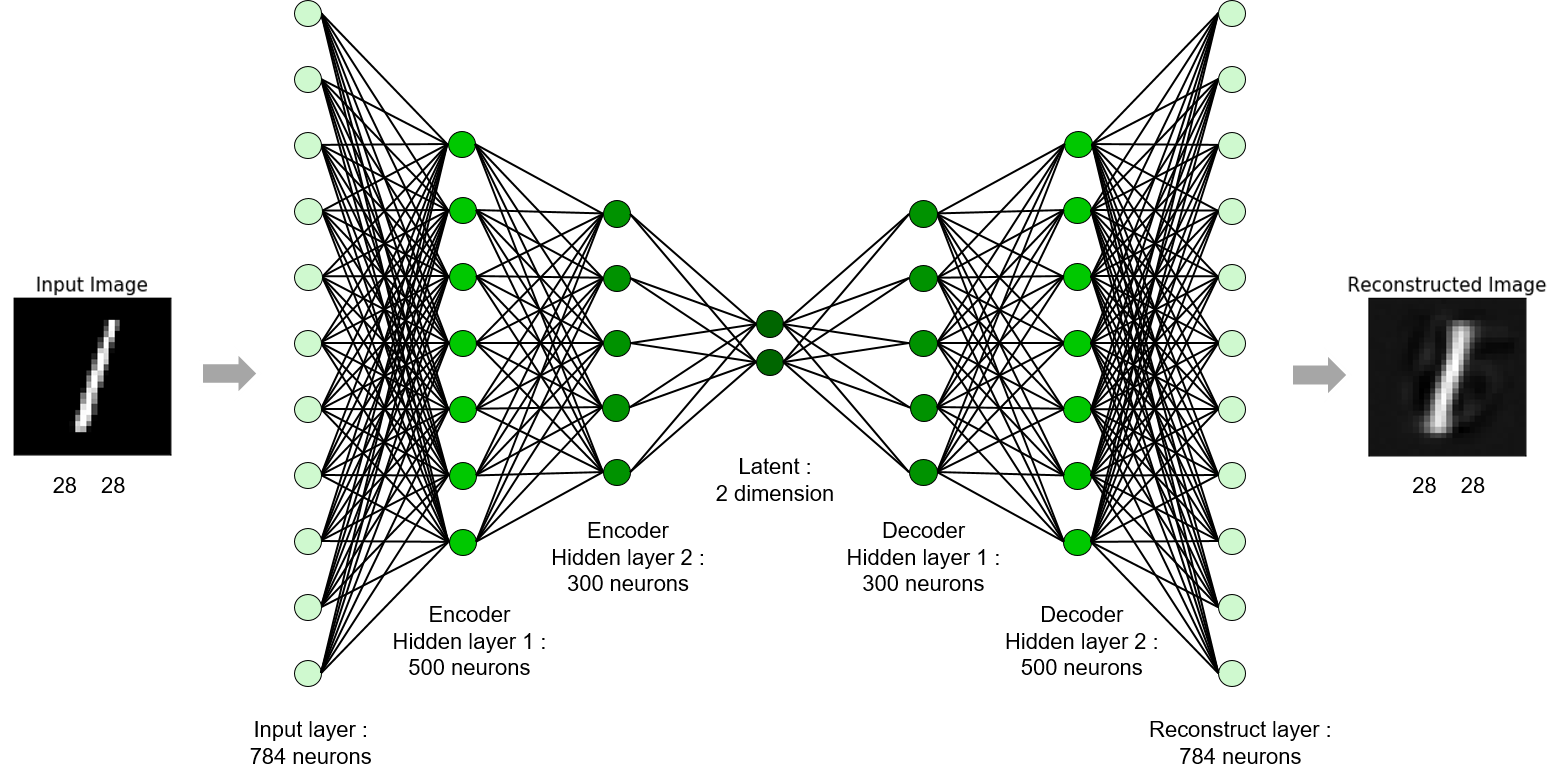
\includegraphics[width=\linewidth]{AE_arch2.png}
  \caption{Autoencoder}
\end{center}
\end{figure}

\subsection{Generatív modellezés}

A generatív modellezés célja, hogy egy adott (felirat mentes) adathalmazból tanulva új adatokat tudjuk generálni ugyanazon eloszlásból, mint amelyből a tanító adatok származnak. Például ha macskákról készült képekkel tanítjuk a modellt, akkor az képes lesz új, korábban nem látott macskákat tartalmazó képeket generálni.

A gyakorlatban használt két legfőbb generatív modell architektúra:
\begin{itemize}
  \item Generative Adversarial Network (GAN)
  \item Variational AutoEncoder (VAE)
\end{itemize}

Az eddigi eredmények azt mutatják, hogy a GAN-ok általában jobb eredményeket adnak, mint a VAE-k, azonban a dolgozatban a VAE-ket fogjuk mélyebben vizsgálni, a GAN-ok csak említés szintjén szerepelnek.

\subsubsection{Generative Adversarial Network (GAN)}

A GAN-ok, tehát ahogy korábban már említettük, olyan neurális hálózatok, melyek képesek az input adathalmaz eloszlásából újabb, véletlenszerű adatokat generálni. Ezt - az autoencoderekhez hasonóan - két egymástól funkcionálisan eltérő neurális háló együttes használatával érjük el a GAN esetében. A két hálót \textit{generátornak} és \textit{diszkriminátornak} nevezzük.

A generátor feladata, hogy egy véletlenszerű kódból előállítson egy adatot az adathalmaz eloszlásából. Az háló inputja tehát egy véletlen zaj, azaz minden input neuronnak egy véletlen értéket adunk meg mind tanításkor, mind kiértékeléskor. Már csak annyi a kérdés, hogy hogyan tudjuk eldönteni az output rétegén megjelenő generált adatról, hogy valóban a kívánt adathalmazból származik-e. Ezen eldöntendő kérdés megválaszolására használjuk a diszkriminátort. A generátor súlyait ezért annak függvényében változtatjuk, hogy a diszkriminátor milyen mértékben tartja valódinak az adatot.

A diszkriminátor feladata tehát, hogy egy adatról eldöntse, valóban az adathalmazból származik-e. Az inputja egy adat, az outpuja pedig mindössze két neuronból áll: egy igen és egy nem választ jelző neuronból. A diszkriminátornak felváltva adunk adatokat az adathalmazból és a generátor kimenetéről, mindkét esetben tudjuk, hogy minek kell lennie a várt eredménynek, így idővel megtanulja megkülönböztetni egymástól a valós és generált adatokat. 

A két hálót tehát párhuzamosan tanítjuk, a generátor folyamatosan megtanul adatokat generálni az adathalmaz eloszlásából, a diszkriminátor pedig folyamatosan megtanulja "leleplezni" a generátort. A modell alapvető felépítését a \ref{gan} ábra személteti.

\begin{figure}[h!]
\begin{center}
  \label{gan}
  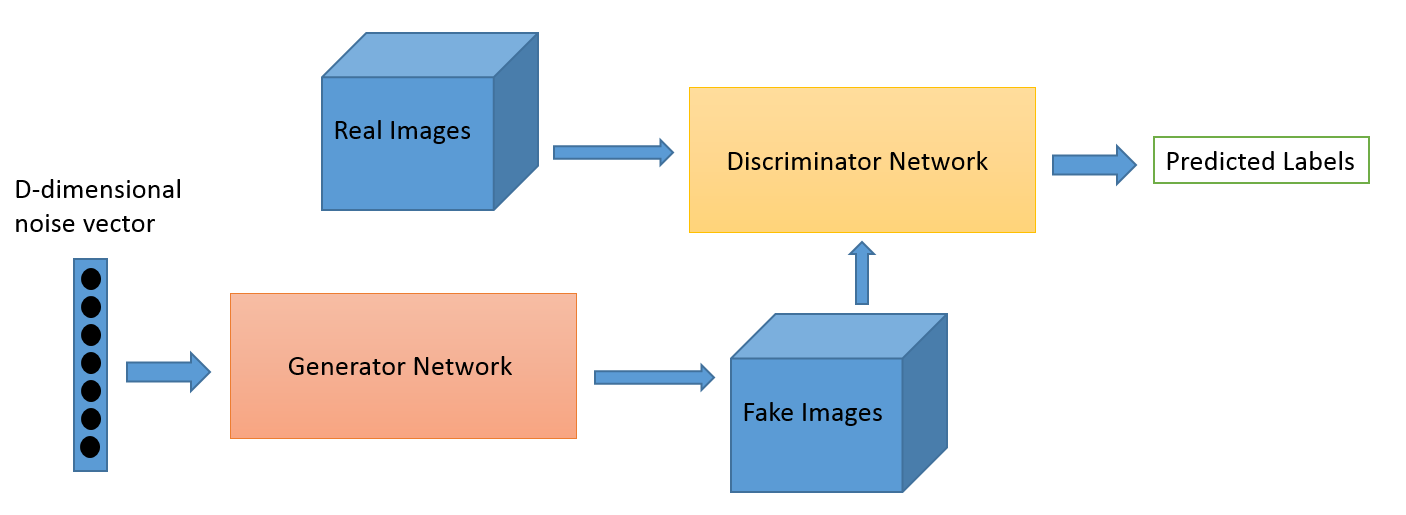
\includegraphics[width=\linewidth]{gan.png}
  \caption{Generative Adversarial Network}
\end{center}
\end{figure}

Az utóbbi néhány évben nagy fejlődésen mentek kereszült a GAN-ok. A \ref{gan_progress} ábrán látható képeket a Celeba adathalmaz (lásd. később) eloszlásából generálták GAN architektúrájú hálókkal. Jól látszik, hogy az elmúlt 5 évben mekkora fejlődésen ment keresztül a szakirány. 

\begin{figure}[h!]
\begin{center}
  \label{gan_progress}
  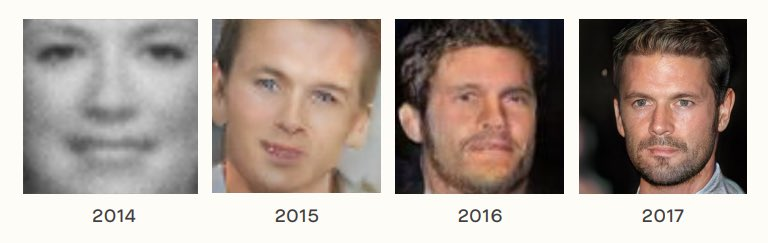
\includegraphics[width=\linewidth]{gan_progress.jpg}
  \caption{GAN modellek fejlődése az elmúlt 4 évben}
\end{center}
\end{figure}

\subsection{Variational AutoEncoder (VAE)}

A variational autoencoderek a GAN-okhoz hasonlóan generatív modellek, azonban a felépítésük - ahogy a nevüben is szerepel -  nagyban hasonlítanak a hagyományos autoencoderekhez.
Első ránézésre az autoencoderek is alkalmasnak tűnnek a generálásra, hiszen a decoder komponensük képes egy látens vektorból előállítani egy adatod, ezért ha egy korábban ismeretlen látens vekorra futtatjuk a decodert, akkor egy új, de mégis hiteles adatot kapnánk. Ez azonban nem működik, mert az autoencoder látens terében a gyakorlatban bizonyos térrészek teljesen érintetlenül maradnak, így a háló nincs felkészülve arra, hogy a látens tér azon szegmenséból generáljon (decode-oljon) adatot.

Ezt a probmémát oldja meg a VAE azzal a trükkel, hogy az encodere nem egy konkrét látens vektort állít elő, mint az adat reprezentációs alakja, hanem egy normáls eloszlást. A variational autoencodereknél valójában ez az eloszlás reprezeltálja az adatot, ami két vektort jelent: egy várható érték és szórás vektort, melyek koordinátánként értendőek a látens vektorra nézve. A tanítás során tehát a decoder (amit a VAE esetében már generátornak is nevezhetünk) inputja egy véletlenszerű vektor ebből az eloszlásból (lásd \ref{vae} ábra).

\begin{figure}[h!]
\begin{center}
  \label{vae}
  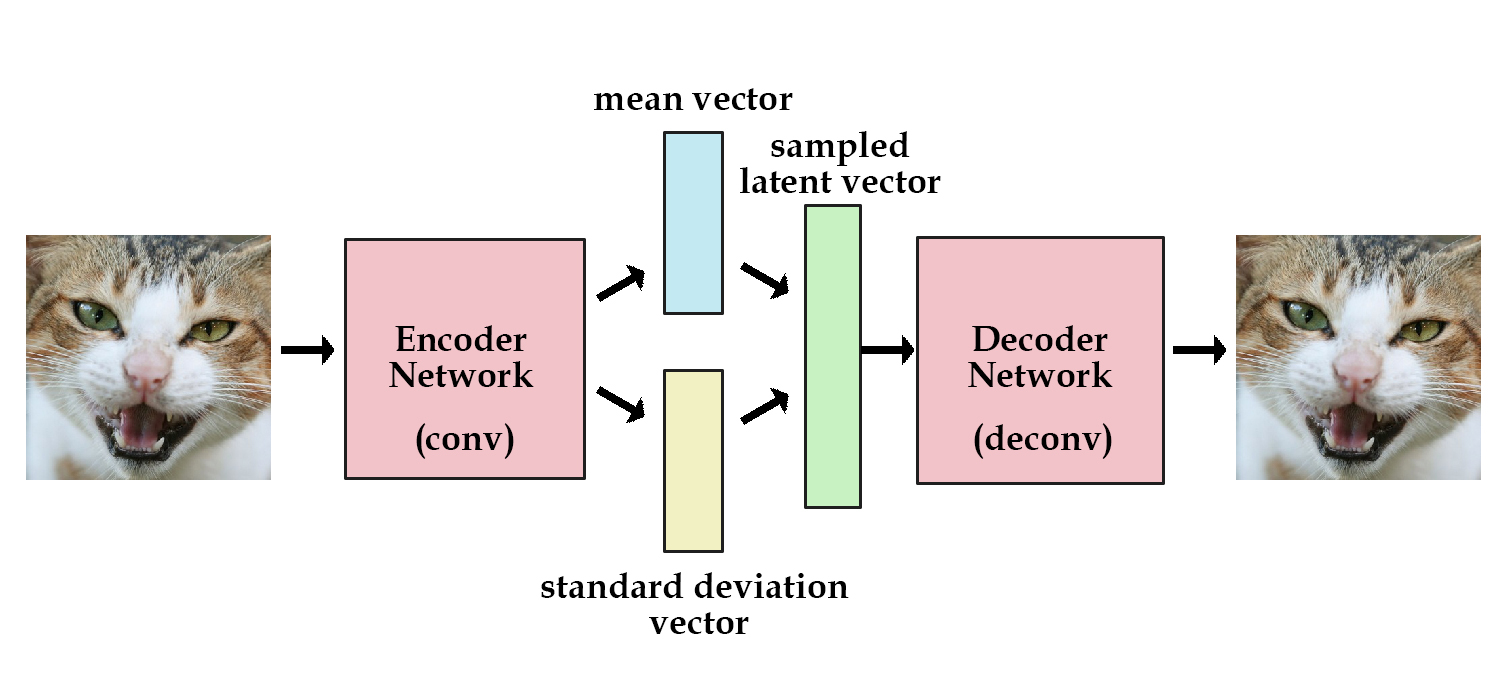
\includegraphics[width=\linewidth]{vae.jpg}
  \caption{GAN modellek fejlődése az elmúlt 4 évben}
\end{center}
\end{figure}

A VAE-k másik fő eltérése a hagyományos autoencoderektől, hogy a backprogpagarion során nem pusztán a rekonstrukció sikeressége szerint javítják a háló súlyait, hanem az KL (Kullback–Leibler) divergencia függvényében is. A KL divergencia nem a kimeneten kapott adatot minősíti, hanem azt, hogy a létrejött eloszlások hogyan helyezkednek el a látens térben. Röviden: az olyan eloszlás halmazokat jutalmazza, amelyek egyenletesen fedik le a látens teret. A tanítás során ezért az adathalmaz adataihoz párosítható látens reprezentációk az egész teret lefedik.

A tanítás végeztével tehát a látens térből bárhonnan választhatunk véletlen vektorokat, azokból valósághű adatotokat fog generálni a decoder.

\subsection{Módosított variational autoencoderek ($\beta$VAE)}

A $\beta$VAE-k nagyon hasonlóak a rendes VAE hálókhoz, mindössze a loss functionben különböznek egymástól. A VAE-k esetében ez a veszteség két komponensből áll: a rekonstrukciós veszteségből és a KL divergenciából. A $\beta$VAE-ben szereplő béta minössze egy konstanst jelent, amely azt határozza meg, hogy a teljes veszteség kiszámításnál a két komponenst milyen súllyal számoljuk, egészen konkrétan a rekonstrukciós veszteségnek mindig $1$, a KL divergenciának pedig $\beta$ a súlya. A rendes VAE hálók tehát valójában $\beta=1$ paraméterű $\beta$VAE-k.

A gyakorlati tapasztalat azt mutatja, hogy az $1$-től eltérő $\beta$-k sok esetben javítanak az eredményeken.

\section{Implementáció}

Lorem ipsum dolor sit amet, consectetur adipiscing elit. Fusce at risus quis nibh dignissim venenatis at id lacus. Aenean cursus erat quis magna tempus, sed ultricies est dictum. Donec sed nisl in ante vestibulum hendrerit a id velit. Phasellus vel erat elit. Morbi eu lobortis sem. Pellentesque at nunc et nibh fringilla mattis eu a diam. Cras mollis convallis vestibulum. Donec at mattis est. Duis cursus enim lorem, eu lobortis ante luctus id. Nullam pellentesque convallis quam. Vestibulum laoreet, dolor sed finibus pulvinar, ante felis convallis lorem, quis pulvinar orci ante at ipsum. Etiam facilisis tincidunt tincidunt. Nunc ipsum purus, egestas eu imperdiet vitae, posuere ut odio. Curabitur consectetur ante quis erat venenatis, eget consectetur mauris viverra.

\subsection{Az alkalmazott szoftverarchitektúra ismertetése}

Lorem ipsum dolor sit amet, consectetur adipiscing elit. Fusce at risus quis nibh dignissim venenatis at id lacus. Aenean cursus erat quis magna tempus, sed ultricies est dictum. Donec sed nisl in ante vestibulum hendrerit a id velit. Phasellus vel erat elit. Morbi eu lobortis sem. Pellentesque at nunc et nibh fringilla mattis eu a diam. Cras mollis convallis vestibulum. Donec at mattis est. Duis cursus enim lorem, eu lobortis ante luctus id. Nullam pellentesque convallis quam. Vestibulum laoreet, dolor sed finibus pulvinar, ante felis convallis lorem, quis pulvinar orci ante at ipsum. Etiam facilisis tincidunt tincidunt. Nunc ipsum purus, egestas eu imperdiet vitae, posuere ut odio. Curabitur consectetur ante quis erat venenatis, eget consectetur mauris viverra.

\subsection{Dsprite és Celeba adathalmazok}

Lorem ipsum dolor sit amet, consectetur adipiscing elit. Fusce at risus quis nibh dignissim venenatis at id lacus. Aenean cursus erat quis magna tempus, sed ultricies est dictum. Donec sed nisl in ante vestibulum hendrerit a id velit. Phasellus vel erat elit. Morbi eu lobortis sem. Pellentesque at nunc et nibh fringilla mattis eu a diam. Cras mollis convallis vestibulum. Donec at mattis est. Duis cursus enim lorem, eu lobortis ante luctus id. Nullam pellentesque convallis quam. Vestibulum laoreet, dolor sed finibus pulvinar, ante felis convallis lorem, quis pulvinar orci ante at ipsum. Etiam facilisis tincidunt tincidunt. Nunc ipsum purus, egestas eu imperdiet vitae, posuere ut odio. Curabitur consectetur ante quis erat venenatis, eget consectetur mauris viverra.

\subsection{Látens reprezentációk strukturáltságának számszerűsítése}

Lorem ipsum dolor sit amet, consectetur adipiscing elit. Fusce at risus quis nibh dignissim venenatis at id lacus. Aenean cursus erat quis magna tempus, sed ultricies est dictum. Donec sed nisl in ante vestibulum hendrerit a id velit. Phasellus vel erat elit. Morbi eu lobortis sem. Pellentesque at nunc et nibh fringilla mattis eu a diam. Cras mollis convallis vestibulum. Donec at mattis est. Duis cursus enim lorem, eu lobortis ante luctus id. Nullam pellentesque convallis quam. Vestibulum laoreet, dolor sed finibus pulvinar, ante felis convallis lorem, quis pulvinar orci ante at ipsum. Etiam facilisis tincidunt tincidunt. Nunc ipsum purus, egestas eu imperdiet vitae, posuere ut odio. Curabitur consectetur ante quis erat venenatis, eget consectetur mauris viverra.

\subsection{Vizualizációs eszközök ismertetése}

Lorem ipsum dolor sit amet, consectetur adipiscing elit. Fusce at risus quis nibh dignissim venenatis at id lacus. Aenean cursus erat quis magna tempus, sed ultricies est dictum. Donec sed nisl in ante vestibulum hendrerit a id velit. Phasellus vel erat elit. Morbi eu lobortis sem. Pellentesque at nunc et nibh fringilla mattis eu a diam. Cras mollis convallis vestibulum. Donec at mattis est. Duis cursus enim lorem, eu lobortis ante luctus id. Nullam pellentesque convallis quam. Vestibulum laoreet, dolor sed finibus pulvinar, ante felis convallis lorem, quis pulvinar orci ante at ipsum. Etiam facilisis tincidunt tincidunt. Nunc ipsum purus, egestas eu imperdiet vitae, posuere ut odio. Curabitur consectetur ante quis erat venenatis, eget consectetur mauris viverra.

\subsection{Kísérletek}

Lorem ipsum dolor sit amet, consectetur adipiscing elit. Fusce at risus quis nibh dignissim venenatis at id lacus. Aenean cursus erat quis magna tempus, sed ultricies est dictum. Donec sed nisl in ante vestibulum hendrerit a id velit. Phasellus vel erat elit. Morbi eu lobortis sem. Pellentesque at nunc et nibh fringilla mattis eu a diam. Cras mollis convallis vestibulum. Donec at mattis est. Duis cursus enim lorem, eu lobortis ante luctus id. Nullam pellentesque convallis quam. Vestibulum laoreet, dolor sed finibus pulvinar, ante felis convallis lorem, quis pulvinar orci ante at ipsum. Etiam facilisis tincidunt tincidunt. Nunc ipsum purus, egestas eu imperdiet vitae, posuere ut odio. Curabitur consectetur ante quis erat venenatis, eget consectetur mauris viverra.

\subsubsection{Tanulási idő hatása}

Lorem ipsum dolor sit amet, consectetur adipiscing elit. Fusce at risus quis nibh dignissim venenatis at id lacus. Aenean cursus erat quis magna tempus, sed ultricies est dictum. Donec sed nisl in ante vestibulum hendrerit a id velit. Phasellus vel erat elit. Morbi eu lobortis sem. Pellentesque at nunc et nibh fringilla mattis eu a diam. Cras mollis convallis vestibulum. Donec at mattis est. Duis cursus enim lorem, eu lobortis ante luctus id. Nullam pellentesque convallis quam. Vestibulum laoreet, dolor sed finibus pulvinar, ante felis convallis lorem, quis pulvinar orci ante at ipsum. Etiam facilisis tincidunt tincidunt. Nunc ipsum purus, egestas eu imperdiet vitae, posuere ut odio. Curabitur consectetur ante quis erat venenatis, eget consectetur mauris viverra.

\subsubsection{$\beta$ hiperparaméter hatása}

Lorem ipsum dolor sit amet, consectetur adipiscing elit. Fusce at risus quis nibh dignissim venenatis at id lacus. Aenean cursus erat quis magna tempus, sed ultricies est dictum. Donec sed nisl in ante vestibulum hendrerit a id velit. Phasellus vel erat elit. Morbi eu lobortis sem. Pellentesque at nunc et nibh fringilla mattis eu a diam. Cras mollis convallis vestibulum. Donec at mattis est. Duis cursus enim lorem, eu lobortis ante luctus id. Nullam pellentesque convallis quam. Vestibulum laoreet, dolor sed finibus pulvinar, ante felis convallis lorem, quis pulvinar orci ante at ipsum. Etiam facilisis tincidunt tincidunt. Nunc ipsum purus, egestas eu imperdiet vitae, posuere ut odio. Curabitur consectetur ante quis erat venenatis, eget consectetur mauris viverra.

\subsubsection{Konvolúciós architektúra hatása}

Lorem ipsum dolor sit amet, consectetur adipiscing elit. Fusce at risus quis nibh dignissim venenatis at id lacus. Aenean cursus erat quis magna tempus, sed ultricies est dictum. Donec sed nisl in ante vestibulum hendrerit a id velit. Phasellus vel erat elit. Morbi eu lobortis sem. Pellentesque at nunc et nibh fringilla mattis eu a diam. Cras mollis convallis vestibulum. Donec at mattis est. Duis cursus enim lorem, eu lobortis ante luctus id. Nullam pellentesque convallis quam. Vestibulum laoreet, dolor sed finibus pulvinar, ante felis convallis lorem, quis pulvinar orci ante at ipsum. Etiam facilisis tincidunt tincidunt. Nunc ipsum purus, egestas eu imperdiet vitae, posuere ut odio. Curabitur consectetur ante quis erat venenatis, eget consectetur mauris viverra.

\begin{thebibliography}{9}

\bibitem{ConvNet}
CS231n Convolutional Neural Networks for Visual Recognition
http://cs231n.github.io/convolutional-networks/

\end{thebibliography}

\end{document}
